% Axis-label correction for rms_vs_re_d.pdf, whose data use 2 pi Omega D.
% Omega is the rotation frequency in Hz throughout the manuscript.
\documentclass[border=0pt]{standalone}
\usepackage{graphicx}
\usepackage{xcolor}
\usepackage{newtxtext,newtxmath}
\begin{document}
\setlength{\unitlength}{1bp}%
\begin{picture}(387.684504,276.714111)
    \put(0,0){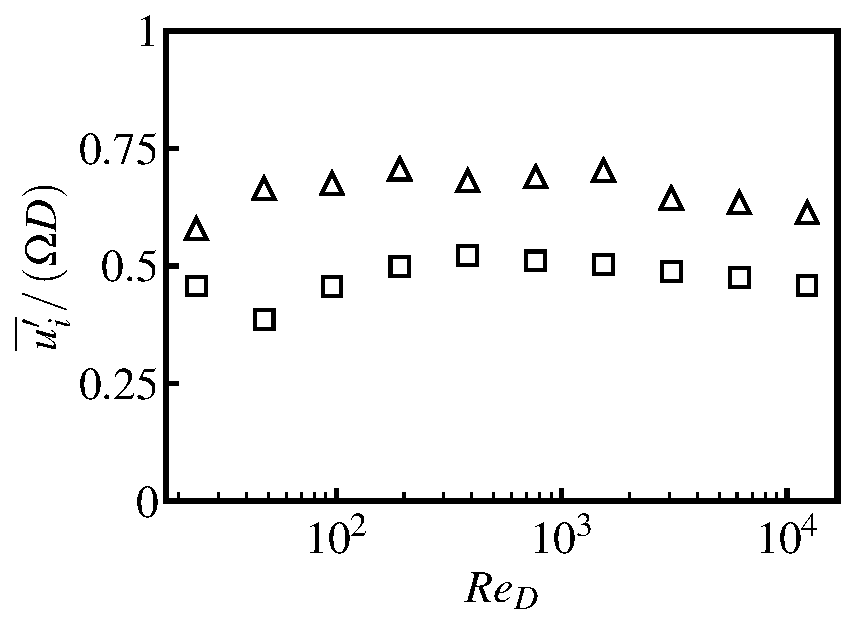
\includegraphics[width=387.684504bp,height=276.714111bp]{rms_vs_re_d.pdf}}%
    \put(0,92){\color{white}\rule{38bp}{140bp}}%
    \put(8,95){\rotatebox{90}{\fontsize{19}{21}\selectfont$\overline{u_i'}/(2\pi\Omega D)$}}%
\end{picture}
\end{document}
